\documentclass[12pt,a4paper]{article}

% Paquetes útiles
\usepackage[utf8]{inputenc}
\usepackage[T1]{fontenc}
\usepackage[spanish]{babel}
\usepackage{geometry}
\usepackage{hyperref}
\usepackage{amsmath, amssymb}
\usepackage{booktabs} % Tablas bonitas
\usepackage{float}    % Control de posición de figuras/tablas
\usepackage{caption}  % Subtítulos de figuras
\usepackage{fancyhdr} % Encabezados y pies de página
\usepackage{graphicx}   % Para incluir imágenes
\usepackage{subcaption} % Para subfiguras
% Márgenes
\geometry{
 a4paper,
 left=25mm,
 right=25mm,
 top=25mm,
 bottom=25mm,
}

% Encabezado y pie de página
\pagestyle{fancy}
\fancyhead[R]{Daniel Camacho Montaño}
\fancyfoot[C]{\thepage}


% Título
\title{Análisis de expresión génica y enriquecimiento funcional en un modelo murino de infección por Staphylococcus aureus bajo tratamiento con Linezolid y Vancomicina}
\author{Daniel Camacho Montaño}
\date{November 2025}


\begin{document}
 
\maketitle

\begin{abstract}
En este trabajo se investigó el efecto de la infección por \textit{Staphylococcus aureus} y de los tratamientos con antibióticos linezolid y vancomicina en la expresión génica de un modelo murino. Se seleccionaron 24 muestras representativas de los grupos experimentales, se procesaron los datos crudos de microarrays Affymetrix y se construyó un objeto \texttt{ExpressionSet}. Tras normalizar los datos mediante RMA y realizar controles de calidad, se identificaron genes diferencialmente expresados mediante modelos lineales ajustados con \texttt{limma}. Posteriormente, se aplicó un análisis de enriquecimiento funcional de Gene Ontology (GO) para evaluar los procesos biológicos implicados en cada contraste experimental. Los resultados muestran que la infección induce respuestas inmunes y metabólicas específicas, mientras que los tratamientos antibióticos generan efectos distintos sobre el transcriptoma, evidenciando la modulación particular de procesos biológicos según el agente utilizado. Este enfoque integral permite caracterizar los cambios funcionales asociados a la infección y a la terapia antibiótica, proporcionando información relevante para la interpretación biológica de los datos transcriptómicos.
\end{abstract}


\newpage

\tableofcontents
\newpage

\section{Introducción y objetivos}

Se utilizó un modelo de ratón para investigar la utilidad de los antibióticos LINEZOLID y VANCOMICINA en la inmunomodulación durante infecciones por \textit{Staphylococcus aureus} resistente a meticilina. La información sobre las muestras y sus condiciones experimentales se encuentra en el fichero \texttt{allTargets.txt}.

El dataset contiene datos de 35 muestras: 15 tomadas antes de la infección, 20 después, 5 correspondientes a las 2 horas que serán eliminadas y 15 a las 24 horas. El objetivo consiste en caracterizar, a través del cambio en la expresión génica, el efecto de la infección y del tratamiento con antibióticos, así como comparar los efectos de ambos tratamientos.

Se plantearon las siguientes comparaciones:

\begin{itemize}
  \item Infectados vs. no infectados sin tratamiento
  \item Infectados vs. no infectados tratados con LINEZOLID
  \item Infectados vs. no infectados tratados con VANCOMICINA
\end{itemize}

Para la obtención de los datos desde Gene Expression Omnibus (GEO), se cargaron los paquetes BioConductor y GEOquery. Los datos del experimento, identificados como \textbf{GSE38531}, se descargaron mediante:

\begin{verbatim}
getGEOSuppFiles("GSE38531", makeDirectory = TRUE)
\end{verbatim}

Esto generó un archivo comprimido \texttt{GSE38531\_RAW.tar} con los datos crudos. La descompresión se realizó con la función \texttt{untar}, especificando el directorio creado para la descarga:

\begin{verbatim}
untar("GSE38531/GSE38531_RAW.tar", exdir = "GSE38531_RAW")
\end{verbatim}

Los archivos descomprimidos corresponden a cada muestra, identificados con el mismo nombre que figura en la columna \texttt{sample} de \texttt{allTargets}, y se almacenan en la carpeta \texttt{GSE38531\_RAW}.

Para simplificar el análisis y reducir el riesgo de intercambio no permitido de información, se eliminaron las muestras correspondientes a las 2 horas (5 muestras) y se seleccionaron aleatoriamente 4 muestras de cada grupo, obteniendo un total de 12 muestras para 3 grupos, o 24 si se considera la selección por interacción de variables (6 grupos experimentales).  

Para realizar el filtrado y el muestreo se definió la función \texttt{filter\_microarray}:

\begin{verbatim}
filter_microarray <- function(allTargets, seed = 39432449) {
  # Configuración de la semilla para reproducibilidad
  set.seed(seed)
  
  # Filtrado de filas donde 'time' no sea 'hour 2'
  filtered <- subset(allTargets, time != "hour 2")
  
  # Creación de la columna 'group' como interacción entre 'infection' y 'agent'
  filtered$group <- interaction(filtered$infection, filtered$agent)
  
  # Selección aleatoria de 4 muestras por grupo
  selected <- do.call(rbind, lapply(split(filtered, filtered$group), 
                function(group_data) {
    if (nrow(group_data) > 4) {
      group_data[sample(1:nrow(group_data), 4), ]
    } else {
      group_data
    }
  }))
  
  # Obtención de los índices originales de las muestras seleccionadas
  original_indices <- match(selected$sample, allTargets$sample)
  
  # Asignación de los índices a los nombres de filas
  rownames(selected) <- paste0(selected$sample, ".", original_indices)
  
  # Eliminación de la columna 'group' y devolución del resultado
  selected$group <- NULL
  return(selected)
}
\end{verbatim}

La función se aplicó al conjunto \texttt{allTargets}, generando un \texttt{data.frame} con 24 muestras seleccionadas, cuyas filas se nombraron según los índices originales del dataset. Las variables categóricas (\texttt{infection}, \texttt{time}, \texttt{agent}) se convirtieron en factores para su posterior análisis.

Esta metodología garantiza que el conjunto de datos utilizado para los análisis contiene una representación balanceada de los grupos experimentales, facilitando comparaciones robustas de los efectos de la infección y de los tratamientos antibióticos.

\subsection{Preparación de los archivos CEL}

Los archivos \texttt{.CEL} de las muestras contienen los datos crudos obtenidos directamente de los experimentos de microarrays Affymetrix. Para generar un \texttt{ExpressionSet}, se descomprimieron previamente los archivos \texttt{.gz} ubicados en \texttt{GSE38531\_RAW} mediante \texttt{lapply}:

\begin{verbatim}
gz_files <- list.files(path = "GSE38531_RAW", pattern = "\\.gz$", 
            full.names = TRUE)
invisible(lapply(gz_files, function(x) gunzip(x, remove = FALSE)))
\end{verbatim}

Una vez descomprimidos, se almacenaron todos los ficheros CEL en una lista denominada \texttt{CEL\_files}. Dado que los nombres de los archivos originales presentan extensiones largas y heterogéneas, se renombraron para mantener únicamente el identificador de la muestra y se generó la lista \texttt{CEL\_files} para reflejar los cambios:

\begin{verbatim}
CEL_files <- list.files(path = "GSE38531_RAW", pattern = "\\.CEL$", 
    full.names = TRUE)
newNames <- paste0(substr(basename(CEL_files), 1, 9), ".CEL")
file.rename(CEL_files, file.path(dirname(CEL_files), newNames))
CEL_files <- list.files(path = "GSE38531_RAW", pattern = "\\.CEL$", 
    full.names = TRUE)
\end{verbatim}

Finalmente, se filtraron los archivos CEL para conservar únicamente aquellos correspondientes a las 24 muestras seleccionadas, eliminando los restantes del directorio:

\begin{verbatim}
celFileNames <- substr(basename(CEL_files), 1, nchar(basename(CEL_files)) - 4)
filesToDelete <- CEL_files[!(celFileNames %in% Targets$sample)]
file.remove(filesToDelete)
\end{verbatim}

La función \texttt{file.remove} devuelve \texttt{TRUE} para cada archivo eliminado, confirmando la eliminación efectiva. El resumen de las muestras seleccionadas es el siguiente:

\begin{verbatim}
sample                     infection       time           agent  
Length:24                  S. aureus USA300:12   hour 0 :12   linezolid :8  
Class :character           uninfected      :12   hour 24:12   untreated :8  
Mode  :character                                      vancomycin:8 
\end{verbatim}

Este procedimiento asegura que el conjunto de datos final contiene únicamente las muestras seleccionadas, debidamente renombradas y categorizadas, permitiendo su uso en análisis posteriores de expresión génica.


\section{Métodos}

\subsection{Creación del ExpressionSet}

Una vez determinadas las muestras que formarán parte del \texttt{ExpressionSet}, se almacenaron en un objeto denominado \texttt{rawData}. Para ello, se especificó el directorio de trabajo y se definieron las rutas para los resultados y los datos de origen:

\begin{verbatim}
workingDir <- getwd()
dataDir <- file.path(workingDir, "GSE38531_RAW")
resultsDir <- file.path(workingDir, "results")
\end{verbatim}

Se cargaron los paquetes \texttt{affy} y \texttt{Biobase} para permitir la lectura de los archivos CEL y la creación del \texttt{ExpressionSet}.

Los nombres de las muestras se asignaron a partir de la variable \texttt{sample} del \texttt{data.frame} \texttt{Targets}. Posteriormente, se creó un objeto \texttt{AnnotatedDataFrame} con la información de las muestras filtradas, incluyendo los metadatos del grupo experimental:

\begin{verbatim}
row.names(Targets) <- Targets$sample
Targets_Annotated <- AnnotatedDataFrame(Targets)
\end{verbatim}

El objeto resultante es un \texttt{AnnotatedDataFrame} con 24 observaciones y 4 variables (\texttt{sample}, \texttt{infection}, \texttt{time} y \texttt{agent}), que contiene la información necesaria para asociar cada muestra con su grupo experimental correspondiente.

Los archivos CEL del directorio \texttt{GSE38531\_RAW}, previamente filtrados mediante la función \texttt{filter\_microarray}, se cargaron en un objeto \texttt{AffyBatch} mediante la función \texttt{ReadAffy}, utilizando \texttt{Targets\_Annotated} para especificar los metadatos:

\begin{verbatim}
CEL_files <- list.files(path = dataDir, pattern = "\\.CEL$", full.names = TRUE)
rawData <- ReadAffy(filenames = CEL_files, phenoData = Targets_Annotated)
\end{verbatim}

A partir del objeto \texttt{AffyBatch}, se extrajeron los datos de expresión (\texttt{exprs}), la información de las muestras (\texttt{pData}) y la información de los genes (\texttt{fData}):

\begin{verbatim}
exprs_data <- exprs(rawData)
pheno_data <- pData(rawData)
feature_data <- fData(rawData)
\end{verbatim}

Con esta información se construyó el \texttt{ExpressionSet}:

\begin{verbatim}
expression_set <- ExpressionSet(assayData = exprs_data,
                                phenoData = AnnotatedDataFrame(pheno_data),
                                featureData = AnnotatedDataFrame(feature_data))
\end{verbatim}

El objeto resultante es un \texttt{ExpressionSet} que contiene los datos de expresión, los metadatos de las muestras y la información de los genes, listo para su uso en análisis posteriores. La estructura del \texttt{ExpressionSet} incluye los slots \texttt{experimentData}, \texttt{assayData}, \texttt{phenoData}, \texttt{featureData}, \texttt{annotation} y \texttt{protocolData}, garantizando que todos los datos y metadatos estén correctamente asociados y etiquetados.

\subsection{Análisis exploratorio y control de calidad}

Se realizó un análisis exploratorio sobre el \texttt{ExpressionSet} para evaluar la distribución de los datos. Los datos de expresión se extrajeron mediante la función \texttt{exprs()} y se construyó un \texttt{boxplot} para visualizar las intensidades de señal de cada muestra:


\begin{figure}[H]
    \centering
    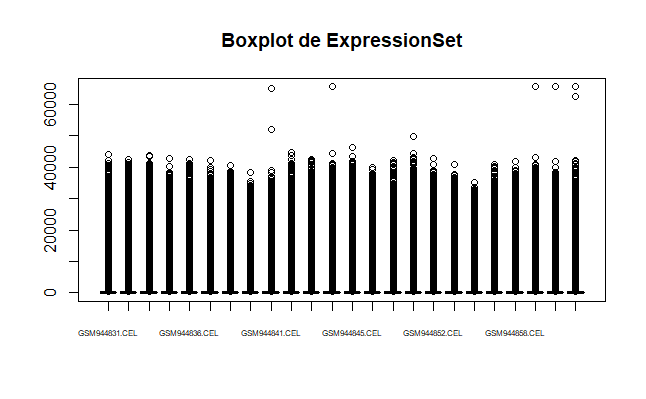
\includegraphics[width=0.8\textwidth]{graphics/boxplot.png}
    \caption{Distribución de las intensidades de expresión de todas las muestras del ExpressionSet.}
    \label{fig:boxplot_expression}
\end{figure}

El \texttt{boxplot} indica que las cajas presentan alturas y posiciones similares entre todas las muestras, sugiriendo que las intensidades crudas no presentan diferencias globales significativas. La presencia de valores atípicos es habitual en datos crudos de microarrays. Para corregir diferencias sistemáticas, se aplicó la normalización RMA (Robust Multi-Array Average), que incluye corrección de \textit{background}, normalización y \textit{summarization}:

\begin{verbatim}
normalized_data <- rma(rawData)
\end{verbatim}

Posteriormente, se generó un \texttt{boxplot} con los datos normalizados, mostrando una distribución homogénea y confirmando la efectividad de la normalización:

\begin{figure}[H]
    \centering
    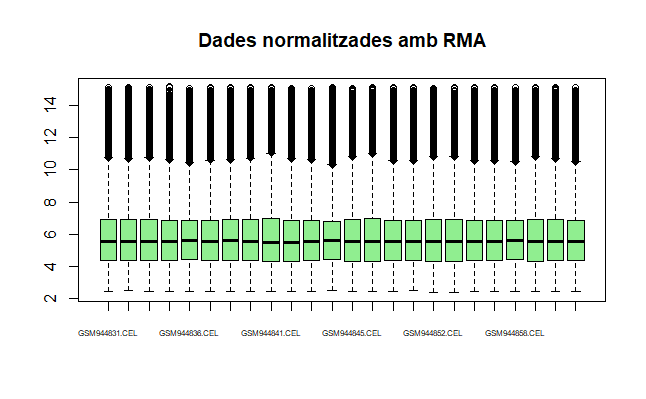
\includegraphics[width=0.8\textwidth]{graphics/boxplot2.png}
    \caption{Distribución de las intensidades de expresión de las muestras tras normalización RMA.}
    \label{fig:boxplot_normalized}
\end{figure}


Se evaluó la calidad de los datos utilizando el paquete \texttt{arrayQualityMetrics}, aplicando el control sobre los datos normalizados y crudos para comparar la mejora tras la normalización:

\begin{verbatim}
library(arrayQualityMetrics)
arrayQualityMetrics(expressionset = normalized_data, 
                    outdir = file.path(resultsDir, "control_calidad"), 
                    force = TRUE)
\end{verbatim}


\begin{figure}[H]
    \centering
    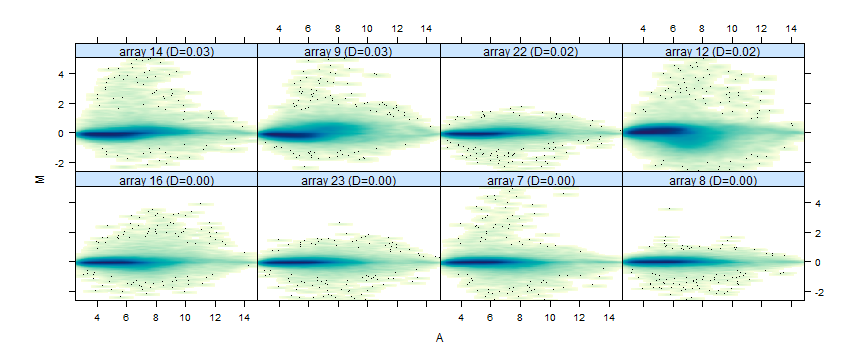
\includegraphics[width=0.7\textwidth]{results/control_calidad/ma.png}
    \caption{MA Plot: Diferencias relativas (M) frente a intensidad promedio (A).}
    \label{fig:ma_plot}
\end{figure}

En este gráfico, los puntos representan las sondas del microarray. Idealmente, los puntos deberían distribuirse simétricamente alrededor de la línea $M=0$. Se observa que la mayoría de los puntos se centra en el eje central, aunque algunos se alejan ligeramente. No se detectan patrones sistemáticos ni estructuras anómalas significativas, lo que indica que los datos normalizados presentan buena calidad.


\begin{figure}[H]
    \centering
    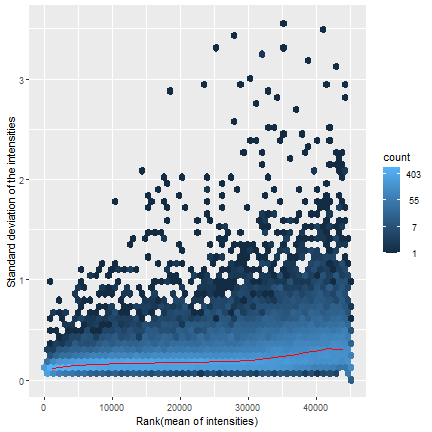
\includegraphics[width=0.7\textwidth]{results/control_calidad/msd.png}
    \caption{MSD Plot: Relación entre intensidad promedio y desviación estándar.}
    \label{fig:msd_plot}
\end{figure}

El MSD Plot permite evaluar cómo varía la desviación estándar en función de la intensidad promedio. La mayoría de los puntos se encuentra concentrada cerca de la base, con algunos valores más dispersos, pero sin variaciones excesivas. La curva roja representa la tendencia general de la desviación estándar. La ligera inclinación observada indica que los datos normalizados mantienen una calidad consistente.


\begin{figure}[H]
    \centering
    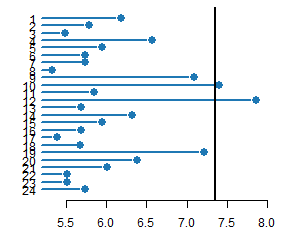
\includegraphics[width=0.7\textwidth]{results/control_calidad/out hm.png}
    \caption{Heatmap de correlación entre muestras (OUT\_HM).}
    \label{fig:out_hm}
\end{figure}

Este heatmap permite evaluar la similitud entre las muestras. Se observa que dos muestras se alejan del agrupamiento principal, lo que indica que presentan patrones de expresión distintos respecto al resto. Esta desviación puede deberse a diferencias biológicas marcadas, baja calidad de la muestra o errores puntuales en la normalización.

\subsubsection{PCA: Análisis de Componentes Principales}
Se realizó un análisis de componentes principales (PCA) para reducir la dimensionalidad de los datos y evaluar posibles agrupamientos por factores experimentales:

\begin{figure}[H]
    \centering
    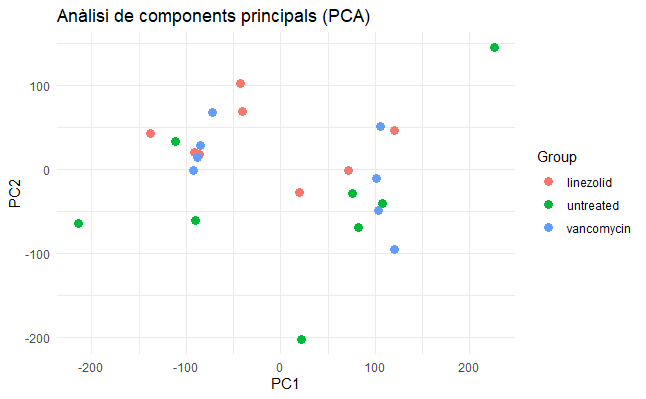
\includegraphics[width=0.7\textwidth]{graphics/PCA.png}
    \caption{Gráfico PCA de los datos normalizados. Cada punto representa una muestra, coloreada según el grupo (\texttt{agent}).}
\end{figure}

No se aprecia un agrupamiento en función del tratamiento (\texttt{agent}), aunque se observa una posible separación en dos grupos no relacionados, lo que podría indicar un efecto \textit{batch} sobre los datos. Para evaluar esto, se generaron tres PCA plots según las variables estudiadas.

\begin{figure}[H]
    \centering
    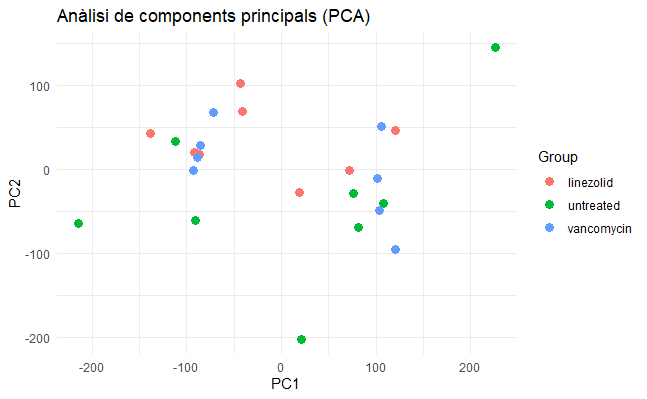
\includegraphics[width=0.7\textwidth]{graphics/PCA_agent.png}
    \caption{PCA según el grupo \texttt{agent}. Cada punto representa una muestra coloreada según el tratamiento.}
    \label{fig:pca_agent}
\end{figure}

\begin{figure}[H]
    \centering
    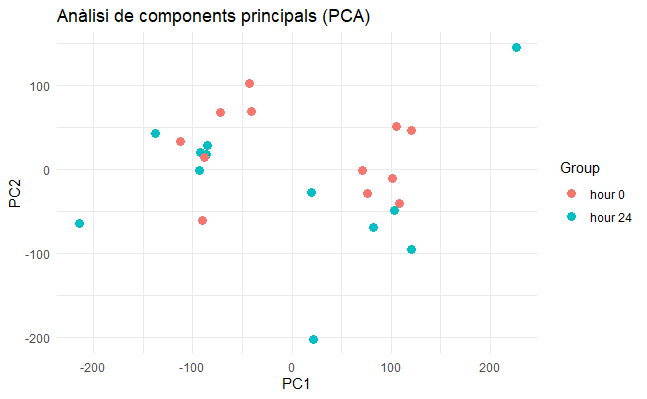
\includegraphics[width=0.7\textwidth]{graphics/PCA_time.png}
    \caption{PCA según la variable \texttt{time}. Cada punto representa una muestra coloreada según el tiempo de muestreo.}
    \label{fig:pca_time}
\end{figure}

\begin{figure}[H]
    \centering
    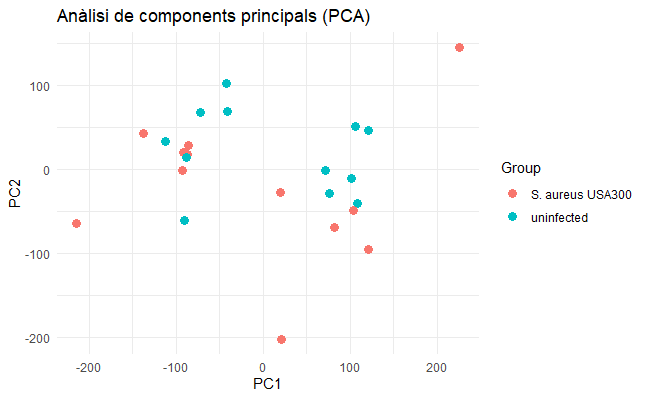
\includegraphics[width=0.7\textwidth]{graphics/PCA_infection.png}
    \caption{PCA según la variable \texttt{infection}. Cada punto representa una muestra coloreada según la condición de infección.}
    \label{fig:pca_infection}
\end{figure}


No se observa un agrupamiento claro debido a alguna de las variables estudiadas, lo que sugiere la existencia de una fuente de variabilidad no contemplada que genera la separación de las muestras en dos bloques. Esto podría deberse a interacciones complejas entre variables o a efectos no lineales que el PCA lineal no logra capturar.

\subsubsection*{Análisis de Variabilidad de Factores de \textit{Batch} (PVCA)}

Se evaluó la variabilidad de las muestras considerando los posibles factores de \textit{batch}, en este caso las variables \texttt{agent}, \texttt{infection} y \texttt{time}, mediante la función \texttt{pvcaBatchAssess} del paquete \texttt{pvca}. Se estableció un umbral del 50\% para la proporción de variabilidad explicada.

\begin{verbatim}
library(pvca)
pData(normalized_data) <- Targets
pct_threshold <- 0.5
batch.factors <- c("agent", "infection","time")
pvcaObj <- pvcaBatchAssess(normalized_data, batch.factors, pct_threshold)
\end{verbatim}

Los resultados se visualizaron en un gráfico de barras, mostrando la proporción de variabilidad explicada por cada factor o interacción de factores:

\begin{figure}[H]
    \centering
    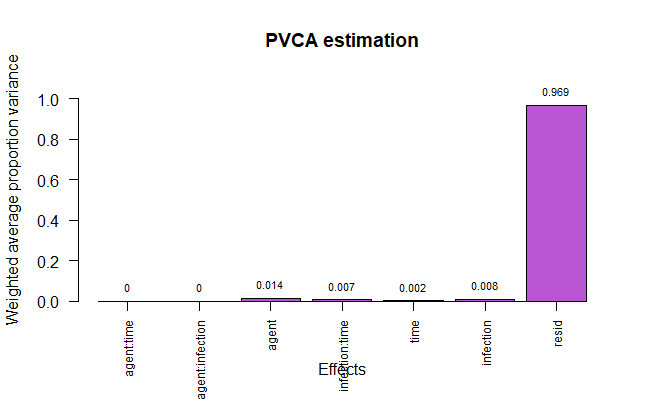
\includegraphics[width=0.7\textwidth]{graphics/PVCA.png}
    \caption{Proporción de variabilidad explicada por los factores \texttt{agent}, \texttt{infection} y \texttt{time} según PVCA.}
\end{figure}

Los resultados indican que los factores considerados no capturan una proporción significativa de la variabilidad observada en los datos, sugiriendo la presencia de fuentes de variabilidad no identificadas o no incluidas en el análisis.

\subsection{Filtro de los Datos}

El filtrado de sondas es un paso crítico en el análisis de microarrays, aunque su aplicación es objeto de debate. En este caso, se decidió conservar únicamente el 10\% de las sondas con mayor variabilidad, eliminando aquellas con variación baja o información redundante.

Se utilizó la función \texttt{nsFilter} del paquete \texttt{genefilter} con los siguientes criterios:

\begin{itemize}
    \item Solo se conservaron sondas con un \textit{Entrez Gene ID} válido (\texttt{require.entrez = TRUE}).
    \item Se eliminaron duplicados de \textit{Entrez Gene ID} (\texttt{remove.dupEntrez = TRUE}).
    \item Se seleccionaron sondas con alta variabilidad, evaluada mediante el \textit{Interquartile Range} (IQR), considerando únicamente aquellas con \texttt{var.cutoff = 0.9}.
    \item Se excluyeron las sondas cuyo identificador comenzaba con \texttt{AFFX}, correspondientes a controles internos o información adicional.
    \item Se aplicó un filtrado por cuantiles para eliminar genes con distribuciones muy sesgadas o valores extremos que pudieran afectar el análisis.
\end{itemize}

El resultado de \texttt{nsFilter} es una lista que contiene los datos filtrados y el nuevo \texttt{ExpressionSet}. El \texttt{ExpressionSet} resultante se almacena en \texttt{filtered\_data}:

\begin{verbatim}
ExpressionSet (storageMode: lockedEnvironment)
assayData: 2048 features, 24 samples 
  element names: exprs 
protocolData
  sampleNames: GSM944831.CEL GSM944833.CEL ... GSM944865.CEL (24
    total)
  varLabels: ScanDate
  varMetadata: labelDescription
phenoData
  sampleNames: GSM944850 GSM944843 ... GSM944862 (24 total)
  varLabels: sample infection ... Group (5 total)
  varMetadata: labelDescription
featureData: none
experimentData: use 'experimentData(object)'
Annotation: mouse4302 
\end{verbatim}

Este procedimiento permite centrar el análisis en las sondas más informativas, eliminando ruido y datos irrelevantes para los análisis posteriores.

\subsection{Construcción de la Matriz de Diseño y de Contraste}

Para definir la matriz de diseño se utilizó el paquete \texttt{limma}. Se creó una nueva variable \texttt{Group} en los metadatos (\texttt{pData}) que combina las variables \texttt{infection} y \texttt{agent} separadas por un guion bajo (\_). Se eliminaron los puntos y se reemplazaron los espacios por guiones bajos para evitar conflictos con los nombres de las variables.

\begin{verbatim}
library(limma)
pData(filtered_data)$Group <- paste(pData(filtered_data)$infection, 
                                    pData(filtered_data)$agent, 
                                    sep = "_")
pData(filtered_data)$Group <- gsub("\\.", "", pData(filtered_data)$Group)
pData(filtered_data)$Group <- gsub(" ", "_", pData(filtered_data)$Group)
\end{verbatim}

A continuación, se creó el objeto \texttt{groups} con la información de la variable \texttt{Group}, y se diseñó un modelo lineal sin intercepto, especificando los niveles de los grupos como nombres de columna de la matriz de diseño.

\begin{verbatim}
groups <- pData(filtered_data)$Group
design <- model.matrix(~0 + factor(groups))
colnames(design) <- levels(factor(groups))
\end{verbatim}

Se verificó la distribución de muestras por grupo experimental y la correcta construcción de la matriz de diseño.

Posteriormente, se construyó la matriz de contrastes mediante la función \texttt{makeContrasts}, definiendo tres comparaciones: uninfected vs S. aureus para cada condición de infección. Es fundamental que los nombres de los contrastes coincidan con los niveles de los grupos definidos en la matriz de diseño.

\begin{verbatim}
contrast_matrix <- makeContrasts(
  Grup1_vs_Grup2 = uninfected_untreated - S_aureus_USA300_untreated,
  Grup1_vs_Grup3 = uninfected_linezolid - S_aureus_USA300_linezolid,
  Grup2_vs_Grup3 = uninfected_vancomycin - S_aureus_USA300_vancomycin,
  levels = design
)
\end{verbatim}

La matriz de contrastes resultante es la siguiente:

\begin{table}[H]
\centering
\begin{tabular}{lccc}
\hline
\textbf{Levels} & \textbf{G1\_vs\_G2} & \textbf{G1\_vs\_G3} & \textbf{G2\_vs\_G3} \\
\hline
S\_aureus\_USA300\_linezolid & 0 & -1 & 0 \\
S\_aureus\_USA300\_untreated & -1 & 0 & 0 \\
S\_aureus\_USA300\_vancomycin & 0 & 0 & -1 \\
uninfected\_linezolid & 0 & 1 & 0 \\
uninfected\_untreated & 1 & 0 & 0 \\
uninfected\_vancomycin & 0 & 0 & 1 \\
\hline
\end{tabular}
\caption{Matriz de contrastes para los diferentes grupos experimentales.}
\end{table}

Esta matriz permitirá realizar los análisis de expresión diferencial entre los grupos definidos.




\subsection{Obtención de los Genes Diferencialmente Expresados}

El análisis de expresión diferencial se realizó aplicando un modelo lineal sobre los datos filtrados (\texttt{filtered\_data}) utilizando la matriz de diseño previamente construida. A continuación, se aplicaron los contrastes definidos y se efectuó una estimación bayesiana para mejorar la estabilidad de las varianzas.

\begin{verbatim}
fit <- lmFit(exprs(filtered_data), design)       # Ajuste del modelo lineal
fit2 <- contrasts.fit(fit, contrast_matrix)      # Aplicar contrastes
fit2 <- eBayes(fit2)                             # Estimación Bayesiana
\end{verbatim}

Los resultados de los contrastes se almacenan en \texttt{fit2}. Para extraer los genes diferencialmente expresados se utilizó la función \texttt{topTable()}, especificando el coeficiente de interés y el método de ajuste de p-valor (\texttt{fdr}):

\begin{verbatim}
Grup1_vs_Grup2 <- topTable(fit2, number=nrow(fit2), coef="Grup1_vs_Grup2", 
        adjust="fdr")
Grup1_vs_Grup3 <- topTable(fit2, number=nrow(fit2), coef="Grup1_vs_Grup3", 
        adjust="fdr")
Grup2_vs_Grup3 <- topTable(fit2, number=nrow(fit2), coef="Grup2_vs_Grup3", 
        adjust="fdr")
\end{verbatim}

\begin{table}[ht]
\centering
\caption{Genes diferencialmente expresados para los tres contrastes principales. Se muestran los 6 primeros genes de cada contraste.}
\begin{tabular}{lrrrrrr}
\hline
\textbf{ProbeID} & \textbf{logFC} & \textbf{AveExpr} & \textbf{t} & \textbf{P.Value} & \textbf{adj.P.Val} & \textbf{B} \\
\hline
\multicolumn{7}{c}{\textbf{Grup1 vs Grup2}} \\
1427084\_a\_at & 0.907 & 7.234 & 2.163 & 0.0413 & 0.9844 & -4.526 \\
1425005\_at & 0.805 & 6.121 & 2.125 & 0.0447 & 0.9844 & -4.529 \\
1460197\_a\_at & -1.908 & 6.686 & -2.117 & 0.0454 & 0.9844 & -4.529 \\
1451536\_at & 0.862 & 9.250 & 2.099 & 0.0471 & 0.9844 & -4.530 \\
1418216\_at & -0.868 & 6.629 & -2.027 & 0.0545 & 0.9844 & -4.535 \\
1449235\_at & 0.908 & 5.738 & 1.988 & 0.0589 & 0.9844 & -4.538 \\
\hline
\multicolumn{7}{c}{\textbf{Grup1 vs Grup3}} \\
1450699\_at & 1.437 & 7.438 & 3.819 & 0.000892 & 0.8108 & -4.405 \\
1436766\_at & -1.202 & 6.300 & -3.056 & 0.00564 & 0.8108 & -4.460 \\
1429808\_at & 1.054 & 6.407 & 2.815 & 0.00988 & 0.8108 & -4.478 \\
1428900\_s\_at & 0.993 & 6.247 & 2.671 & 0.0137 & 0.8108 & -4.489 \\
1450919\_at & 0.972 & 12.968 & 2.607 & 0.0158 & 0.8108 & -4.493 \\
1425814\_a\_at & 1.404 & 8.631 & 2.584 & 0.0167 & 0.8108 & -4.495 \\
\hline
\multicolumn{7}{c}{\textbf{Grup2 vs Grup3}} \\
1427161\_at & 1.518 & 7.305 & 3.427 & 0.00232 & 0.9999 & -4.433 \\
1417133\_at & -1.506 & 6.103 & -3.051 & 0.00570 & 0.9999 & -4.460 \\
1426817\_at & 0.990 & 10.462 & 2.995 & 0.00651 & 0.9999 & -4.465 \\
1453220\_at & 1.142 & 6.848 & 2.912 & 0.00790 & 0.9999 & -4.471 \\
1452661\_at & 1.283 & 12.367 & 2.912 & 0.00790 & 0.9999 & -4.471 \\
1433623\_at & 1.090 & 6.659 & 2.884 & 0.00843 & 0.9999 & -4.473 \\
\hline
\end{tabular}
\end{table}




En este análisis, ningún contraste arrojó un p-valor ajustado significativo, probablemente debido al efecto batch y a la variabilidad no explicada identificada previamente. Para continuar con el análisis, se consideraron los p-valores sin ajustar, reconociendo que estos no corrigen el error de tipo I asociado a las pruebas múltiples:

\begin{verbatim}
g1_vs_g2 <- Grup1_vs_Grup2[Grup1_vs_Grup2$P.Value < 0.05, ]
g1_vs_g3 <- Grup1_vs_Grup3[Grup1_vs_Grup3$P.Value < 0.05, ]
g2_vs_g3 <- Grup2_vs_Grup3[Grup2_vs_Grup3$P.Value < 0.05, ]
\end{verbatim}




Estos subconjuntos contienen los genes con p-valor menor a 0.05, y constituyen la base para posteriores análisis funcionales o de visualización.

\begin{table}[ht]
\centering
\caption{Genes diferencialmente expresados con P.Value $<$ 0.05 para los tres contrastes principales. Se muestran los 6 primeros genes de cada contraste.}
\begin{tabular}{lrrrrrr}
\toprule
\textbf{ProbeID} & \textbf{logFC} & \textbf{AveExpr} & \textbf{t} & \textbf{P.Value} & \textbf{adj.P.Val} & \textbf{B} \\
\midrule
\multicolumn{7}{c}{\textbf{g1 vs g2}} \\
1427084\_a\_at & 0.907 & 7.234 & 2.163 & 0.04132 & 0.98438 & -4.526 \\
1425005\_at & 0.805 & 6.121 & 2.125 & 0.04466 & 0.98438 & -4.529 \\
1460197\_a\_at & -1.908 & 6.686 & -2.117 & 0.04541 & 0.98438 & -4.529 \\
1451536\_at & 0.862 & 9.250 & 2.099 & 0.04707 & 0.98438 & -4.530 \\
\midrule
\multicolumn{7}{c}{\textbf{g1 vs g3}} \\
1450699\_at & 1.437 & 7.438 & 3.819 & 0.000892 & 0.81084 & -4.405 \\
1436766\_at & -1.202 & 6.300 & -3.056 & 0.005642 & 0.81084 & -4.460 \\
1429808\_at & 1.054 & 6.407 & 2.815 & 0.009882 & 0.81084 & -4.478 \\
1428900\_s\_at & 0.993 & 6.247 & 2.671 & 0.01370 & 0.81084 & -4.489 \\
1450919\_at & 0.972 & 12.968 & 2.607 & 0.01582 & 0.81084 & -4.493 \\
1425814\_a\_at & 1.404 & 8.631 & 2.584 & 0.01665 & 0.81084 & -4.495 \\
\midrule
\multicolumn{7}{c}{\textbf{g2 vs g3}} \\
1427161\_at & 1.518 & 7.305 & 3.427 & 0.002324 & 0.99989 & -4.433 \\
1417133\_at & -1.506 & 6.103 & -3.051 & 0.005702 & 0.99989 & -4.460 \\
1426817\_at & 0.990 & 10.462 & 2.995 & 0.006510 & 0.99989 & -4.465 \\
1453220\_at & 1.142 & 6.848 & 2.912 & 0.007897 & 0.99989 & -4.471 \\
1452661\_at & 1.283 & 12.367 & 2.912 & 0.007904 & 0.99989 & -4.471 \\
1433623\_at & 1.090 & 6.659 & 2.884 & 0.008432 & 0.99989 & -4.473 \\
\bottomrule
\end{tabular}
\end{table}



\subsection{Anotación de los Genes}

El \texttt{ExpressionSet} utilizado está basado en el Affymetrix Mouse Genome 430 2.0 Array, como se indica en \texttt{Annotation=mouse4302}. En las tablas obtenidas mediante \texttt{topTable}, las filas se identifican con los identificadores de Affymetrix, accesibles mediante \texttt{rownames()}. Adicionalmente, el proyecto GEO proporciona un archivo de anotaciones (\texttt{GPL1261.annot}) que incluye información sobre los genes, como el símbolo (\texttt{Symbol}), el identificador \texttt{Entrez} y detalles sobre la actividad biológica.

Para realizar el mapeo de sondas a identificadores \texttt{ENTREZID} se utilizó el paquete de anotaciones \texttt{mouse4302.db} junto con la función \texttt{mapIds}, considerando que las claves originales están en formato \texttt{PROBEID}:

\begin{verbatim}
library(mouse4302.db)

# Mapeado del primer contraste
mapped_ids12 <- mapIds(
  mouse4302.db,
  keys = rownames(g1_vs_g2),
  column = "ENTREZID", 
  keytype = "PROBEID",
  multiVals = "first"
)

# Mapeado del segundo contraste
mapped_ids13 <- mapIds(
  mouse4302.db,
  keys = rownames(g1_vs_g3),
  column = "ENTREZID", 
  keytype = "PROBEID",
  multiVals = "first"
)

# Mapeado del tercer contraste
mapped_ids23 <- mapIds(
  mouse4302.db,
  keys = rownames(g2_vs_g3),
  column = "ENTREZID", 
  keytype = "PROBEID",
  multiVals = "first"
)
\end{verbatim}

Posteriormente, los identificadores \texttt{ENTREZID} se añadieron como una nueva columna en los resultados de cada contraste:

\begin{verbatim}
g1_vs_g2$ENTREZID <- mapped_ids12
g1_vs_g3$ENTREZID <- mapped_ids13
g2_vs_g3$ENTREZID <- mapped_ids23
\end{verbatim}

De este modo, la lista de genes significativos incluye ahora la columna \texttt{ENTREZID}, proporcionando el identificador estándar de cada gen para análisis posteriores.

\subsection{Análisis de la Significación Biológica}

Cada lista de genes contiene aquellos que se han expresado diferencialmente en cada contraste. El análisis de la significación biológica permite identificar genes que podrían tener un impacto funcional relevante o que podrían estar implicados en procesos biológicos clave.

Se realizó un análisis de enriquecimiento de \textit{Gene Ontology} utilizando el paquete \texttt{clusterProfiler} y la función \texttt{enrichGO}. En este análisis se especificaron los identificadores de los genes (\texttt{gene}), la base de anotaciones utilizada (\texttt{OrgDb}), el tipo de identificador (\texttt{keyType}) y la ontología de interés (\texttt{ont}):

\begin{verbatim}
library(clusterProfiler)

enrich_result12 <- enrichGO(
  gene = g1_vs_g2$ENTREZID,
  OrgDb = mouse4302.db,
  keyType = "ENTREZID",
  ont = "BP",
  pAdjustMethod = "BH"
)

enrich_result13 <- enrichGO(
  gene = g1_vs_g3$ENTREZID,
  OrgDb = mouse4302.db,
  keyType = "ENTREZID",
  ont = "BP",
  pAdjustMethod = "BH"
)

enrich_result23 <- enrichGO(
  gene = g2_vs_g3$ENTREZID,
  OrgDb = mouse4302.db,
  keyType = "ENTREZID",
  ont = "BP",
  pAdjustMethod = "BH"
)
\end{verbatim}

Para visualizar los resultados del análisis de GO, se generaron diagramas de puntos (\texttt{dotplot}) para cada contraste:

\begin{figure}[H]
    \centering
    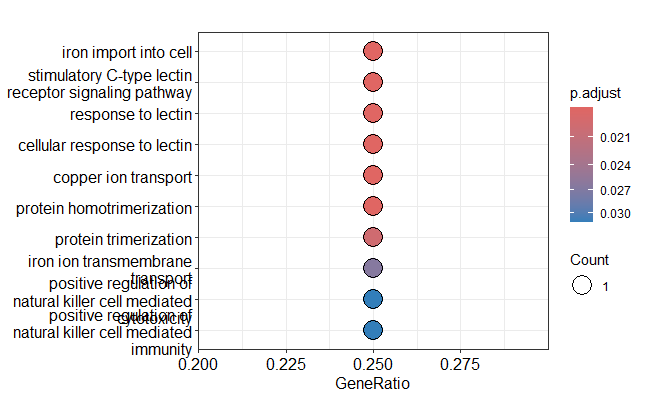
\includegraphics[width=0.8\textwidth]{graphics/GO_g1_vs_g2.png}
    \caption{Enriquecimiento GO: g1 vs g2 (untreated). Este gráfico muestra los términos GO más significativos con su respectiva proporción de genes (GeneRatio) y el p-valor ajustado.}
    \label{fig:go_g1_g2}
\end{figure}

\begin{figure}[H]
    \centering
    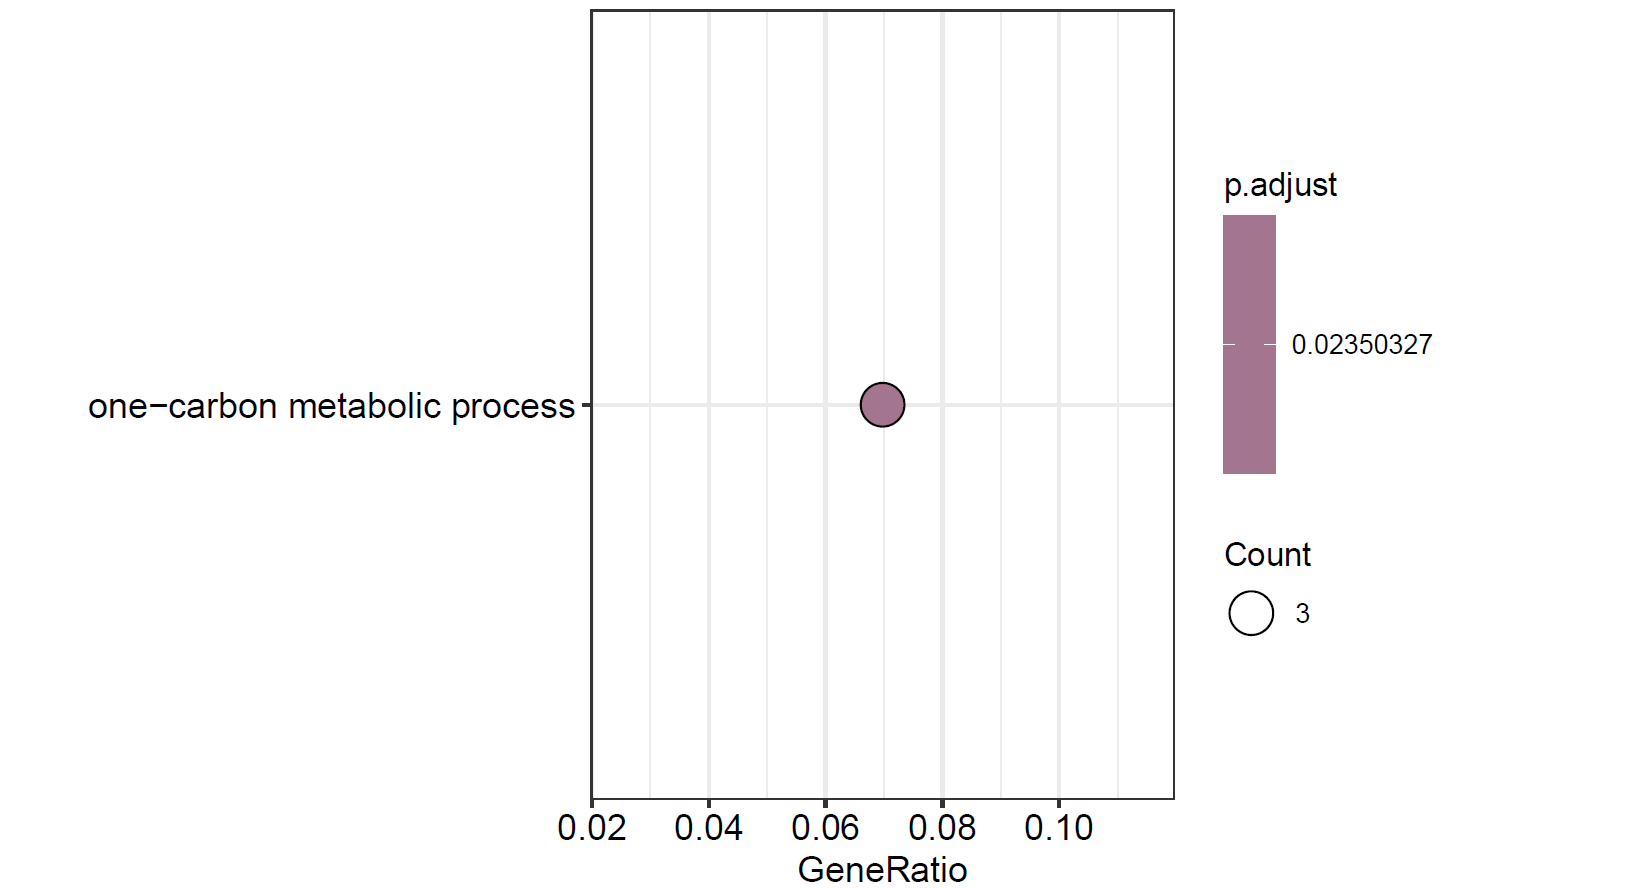
\includegraphics[width=0.8\textwidth]{graphics/GO_g1_vs_g3.png}
    \caption{Enriquecimiento GO: g1 vs g3 (linezolid). Este gráfico muestra los términos GO más significativos con su respectiva proporción de genes (GeneRatio) y el p-valor ajustado.}
    \label{fig:go_g1_g3}
\end{figure}

\begin{figure}[H]
    \centering
    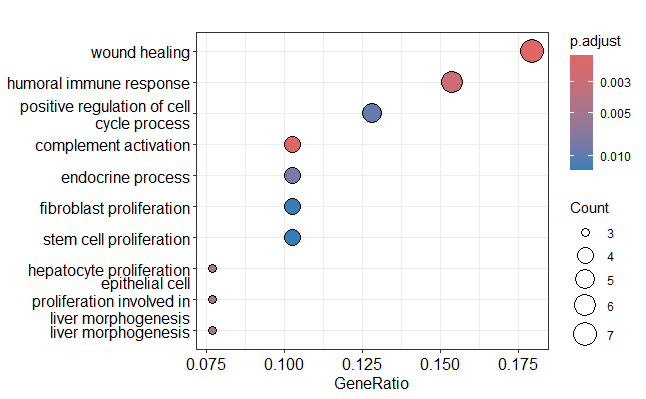
\includegraphics[width=0.8\textwidth]{graphics/GO_g2_vs_g3.png}
    \caption{Enriquecimiento GO: g2 vs g3 (vancomycin). Este gráfico muestra los términos GO más significativos con su respectiva proporción de genes (GeneRatio) y el p-valor ajustado.}
    \label{fig:go_g2_g3}
\end{figure}




Estos gráficos permiten identificar los términos de \textit{Gene Ontology} más enriquecidos en cada lista de genes, facilitando la interpretación biológica de los resultados.








\section{Resultados}

Los tres gráficos generados representan los resultados de enriquecimiento de \textit{Gene Ontology} (GO) y reflejan diferencias entre las condiciones experimentales. En cada gráfico, el \textit{GeneRatio} indica la proporción de genes de la lista del contraste asociados con cada término GO.

En el primer gráfico (untreated) se observan múltiples términos GO relacionados con procesos biológicos como respuesta inmune, cicatrización y desarrollo hepático. Todos los procesos presentan un \textit{GeneRatio} similar, aunque algunos muestran un p-valor ajustado más significativo que otros. Esto indica que los genes diferencialmente expresados se deben principalmente a la infección con \textit{S. aureus}, dado que no existe otro tratamiento en esta condición.

En el segundo gráfico (linezolid) únicamente aparece un término GO, correspondiente al \textit{One-carbon metabolic process}, con un \textit{GeneRatio} bajo y un p-valor ajustado significativo. Este contraste evalúa los efectos del tratamiento con linezolid en presencia de la infección bacteriana, sugiriendo un efecto específico del antibiótico sobre el metabolismo del carbono.

En el tercer gráfico (vancomycin) se destacan procesos relacionados con transporte de hierro, respuesta de lectinas y transporte iónico, entre otros términos con \textit{GeneRatio} elevado. Estos términos reflejan mecanismos específicos de acción del antibiótico o respuestas celulares frente a la infección, mostrando los efectos particulares de la combinación de infección y tratamiento con vancomicina.

\end{document}